\section{NUMA aware scheduler design}
In order to easily experiment with NUMA-aware task scheduling, we
implemented our own basic NUMA task scheduler. 
%
We call this scheduler ``Nas'' (NUMA Aware Scheduler) in the remainder of this paper.

Nas design is similar to TBB, in that, tasks are objects containing an execute method and some extra information such as dependencies.
%
Each task have a NUMA node affinity property to allow Nas scheduling tasks with the best affinity.
%
This NUMA node affinity can be strict or not.
%
In strict mode, the tasks can only be executed on one NUMA node.
%
In flexible mode, tasks are executed in priority on the specified NUMA, but can also be executed somewhere else if needed.

In Nas, threads of the same NUMA node share the same deque of tasks, unlike other runtimes that use one deque per thread.
%
When a task becomes available, it is put into the container corresponding to its NUMA affinity if set, otherwise a round robin algorithm is used by default.
%
Because of thread concurrency over the container, we didn't choose a simple deque but rather an optimized structure which allows multiple operations at the same time.

Nas also provides control over data allocation and distribution
among NUMA banks, as well as memory block moves among NUMA banks.

Nas and Taggre are designed to cooperate together, with Taggre being responsible for the DAG preprocessing, and Nas acting as the
runtime back-end. 
%
Both tools also cooperate together in controlling the placement of
tasks on the NUMA platform: The aggregation operator is called using the Front algorithm with the number of NUMA nodes as parameter. (TODO: ref agg operator)

%-------------------------------
\subsection{NUMA helpers}
\label{NUMA_helper}
Nas has some NUMA helpers for allocation.
%
The first helper is a function to allocate data and distribute it over all NUMA banks.
%
This is equivalent to starting a static parallel for with OpenMP and First Touch policy activated, but in our case we have simplified this through a single function call.
%
In linear algebra, this helper is mainly useful for vector allocation.

The second helper is a function to move data between NUMA banks.
%
The user registers the piece of data and where he wants to move it.
%
This helper is basically a wrapper for the {\em move\_pages} system call.
%
It automatically splits memory address and size into
a set of memory addresses aligned to page boundaries.
%
This helper can be combined with Taggre to distribute data by taking into account data access over computation time.


Thus, using Nas in conjunction with Taggre is a very convenient way to manage NUMA seamlessly in a task driven parallelization.
%
Indeed, we provide a single function that uses the Taggre DAG to perform an allocate or move memory pages of the data in order to balance the work between sockets in accordance with the DAG.
%
The task affinity with the sockets where its data are allocated is then used by the scheduler to minimize the NUMA penalties.
%
More details are given in the next section.

%-------------------------------
\subsection{Nas with Taggre}
In order to optimize NUMA memory distribution, one can use the DAG of Taggre, and Nas as runtime.
%
In most cases, tasks have data from other tasks to read in input and produce data for other tasks in output.
%
By distributing tasks over NUMA nodes, we can indirectly distribute
the data production.
%
Usually, the NUMA penalty of a write access is worst than the NUMA penalty of a read access.
%
The tasks distribution is done with the Front algorithm
and the number of NUMA nodes as parameter (Fig. \ref{fig:distrib_numa}).

Then we need to match the NUMA locality of data with the NUMA affinity of tasks which use it by moving physical pages on the right NUMA bank.
%
To do this, we simulate an execution of the DAG with a user defined function.
%
This function is called for each task and must register data write in the task to express that it should be brought them closer.

In the case of GMRES, we distribute the row of the matrix following the DAG.
%
All vectors used during triangular solve are allocated using the first NUMA helper.


\begin{figure}[!ht]
  \centering
  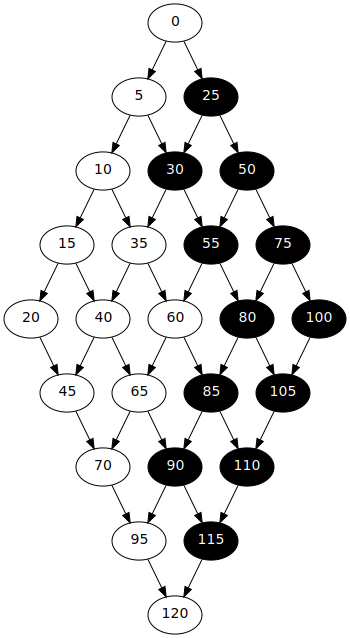
\includegraphics[width=2.5in]{numa_distrib}
  \caption{Distribution of tasks between 2 NUMA nodes, in white tasks of node 1, in black tasks of node 2}
  \label{fig:distrib_numa}
\end{figure}

